\documentclass[tikz]{standalone}

\usepackage{tikz}
\usepackage[fontsize=14pt]{fontsize}
\usetikzlibrary{matrix,positioning}

\tikzset{ 
table/.style={
  matrix of nodes,
  row sep=-\pgflinewidth,
  column sep=-\pgflinewidth,
  nodes={
    rectangle,draw,
    text width=0.5cm,
    %minimum width=0.75cm,
    %minimum height=0.75cm,
    align=center},
  text depth=0.125cm,
  text height=0.25cm,
  nodes in empty cells,
  outer sep=0cm,
  },
%texto/.style={font=\footnotesize\sffamily},
%title/.style={font=\small\sffamily}
}

\begin{document}
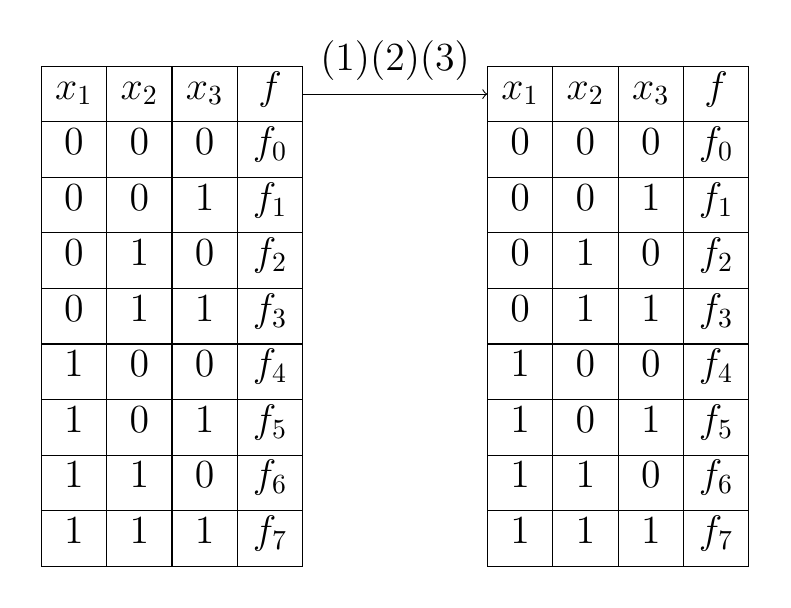
\begin{tikzpicture}
    \matrix (f) [table]
    {
        $x_1$ & $x_2$ & $x_3$ & $f$ \\
        0 & 0 & 0 & $f_0$ \\
        0 & 0 & 1 & $f_1$ \\
        0 & 1 & 0 & $f_2$ \\
        0 & 1 & 1 & $f_3$ \\
        1 & 0 & 0 & $f_4$ \\
        1 & 0 & 1 & $f_5$ \\
        1 & 1 & 0 & $f_6$ \\
        1 & 1 & 1 & $f_7$ \\
    };
    \matrix (g) [table, right=2cm of f.east, node distance=2cm]
    {
      $x_1$ & $x_2$ & $x_3$ & $f$ \\
      0 & 0 & 0 & $f_0$ \\
      0 & 0 & 1 & $f_1$ \\
      0 & 1 & 0 & $f_2$ \\
      0 & 1 & 1 & $f_3$ \\
      1 & 0 & 0 & $f_4$ \\
      1 & 0 & 1 & $f_5$ \\
      1 & 1 & 0 & $f_6$ \\
      1 & 1 & 1 & $f_7$ \\
    };
    \draw [->] (f-1-4.east) -- node [above] {$(1)(2)(3)$} (g-1-1.west);
\end{tikzpicture}

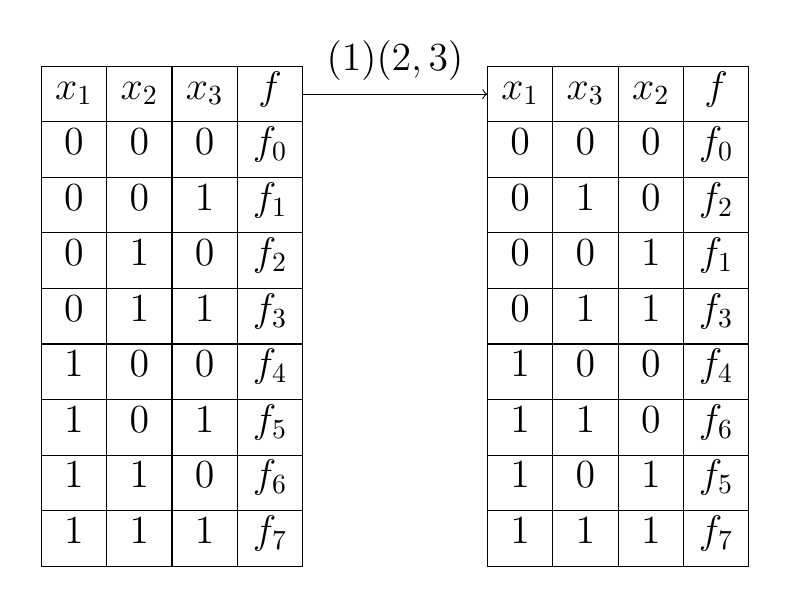
\begin{tikzpicture}
    \matrix (f) [table]
    {
        $x_1$ & $x_2$ & $x_3$ & $f$ \\
        0 & 0 & 0 & $f_0$ \\
        0 & 0 & 1 & $f_1$ \\
        0 & 1 & 0 & $f_2$ \\
        0 & 1 & 1 & $f_3$ \\
        1 & 0 & 0 & $f_4$ \\
        1 & 0 & 1 & $f_5$ \\
        1 & 1 & 0 & $f_6$ \\
        1 & 1 & 1 & $f_7$ \\
    };
    \matrix (g) [table, right=2cm of f.east, node distance=2cm]
    {
      $x_1$ & $x_3$ & $x_2$ & $f$ \\
      0 & 0 & 0 & $f_0$ \\
      0 & 1 & 0 & $f_2$ \\
      0 & 0 & 1 & $f_1$ \\
      0 & 1 & 1 & $f_3$ \\
      1 & 0 & 0 & $f_4$ \\
      1 & 1 & 0 & $f_6$ \\
      1 & 0 & 1 & $f_5$ \\
      1 & 1 & 1 & $f_7$ \\
    };
    \draw [->] (f-1-4.east) -- node [above] {$(1)(2, 3)$} (g-1-1.west);
\end{tikzpicture}

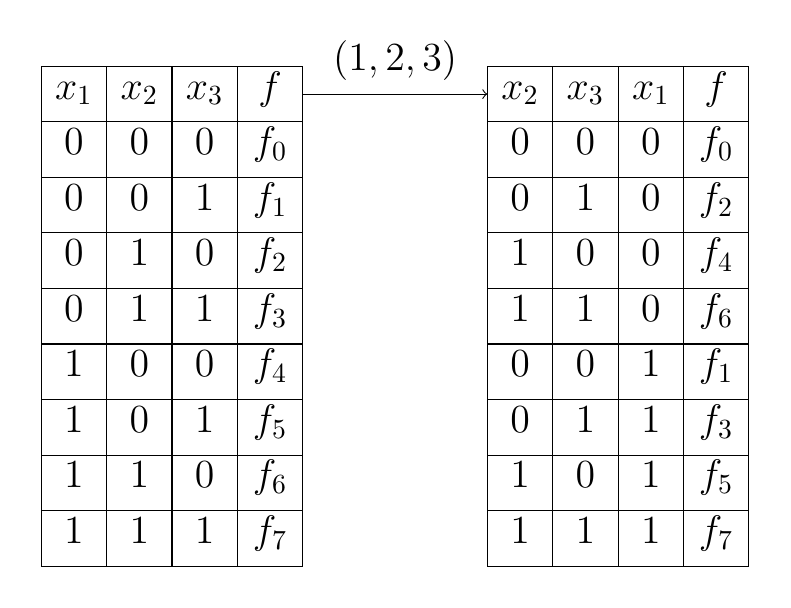
\begin{tikzpicture}
    \matrix (f) [table]
    {
        $x_1$ & $x_2$ & $x_3$ & $f$ \\
        0 & 0 & 0 & $f_0$ \\
        0 & 0 & 1 & $f_1$ \\
        0 & 1 & 0 & $f_2$ \\
        0 & 1 & 1 & $f_3$ \\
        1 & 0 & 0 & $f_4$ \\
        1 & 0 & 1 & $f_5$ \\
        1 & 1 & 0 & $f_6$ \\
        1 & 1 & 1 & $f_7$ \\
    };
    \matrix (g) [table, right=2cm of f.east, node distance=2cm]
    {
      $x_2$ & $x_3$ & $x_1$ & $f$ \\
      0 & 0 & 0 & $f_0$ \\
      0 & 1 & 0 & $f_2$ \\
      1 & 0 & 0 & $f_4$ \\
      1 & 1 & 0 & $f_6$ \\
      0 & 0 & 1 & $f_1$ \\
      0 & 1 & 1 & $f_3$ \\
      1 & 0 & 1 & $f_5$ \\
      1 & 1 & 1 & $f_7$ \\
    };
    \draw [->] (f-1-4.east) -- node [above] {$(1, 2, 3)$} (g-1-1.west);
\end{tikzpicture}
\end{document}